%\documentclass[letterpaper,12pt,dvips]{article}
\documentclass[letterpaper,12pt]{article}

\usepackage{latexsym}
\usepackage{fancybox}
\usepackage{graphicx}
\usepackage{natbib}
\usepackage{color}
\usepackage{amsmath}
\usepackage{amssymb}
\usepackage{ulem}
\usepackage{float}
\usepackage{here}
\usepackage{multicol}
\usepackage{caption}
\usepackage{sidecap}

\pretolerance=10000
\textwidth=6.5in
\textheight=8.9in
\voffset = -0.3in
\topmargin=0.0in
\headheight=0.00in
\hoffset = 0.0in
\headsep=0.00in
\oddsidemargin=0in
\evensidemargin=0in
\parindent=2em
\parskip=1.5ex

\DeclareMathAlphabet{\mathsc}{OT1}{cmr}{m}{sc}
\def\testbx{bx}
\DeclareRobustCommand{\ion}[2]{
\relax\ifmmode
\ifx\testbx\f@series
{\mathbf{#1\,\mathsc{#2}}}\else
{\mathrm{#1\,\mathsc{#2}}}\fi
\else\textup{#1\,{\mdseries\textsc{#2}}}
\fi}

\newenvironment{my_itemize}{
\begin{itemize}
  \setlength{\itemsep}{1pt}
  \setlength{\parskip}{0pt}
  \setlength{\parsep}{0pt}}{\end{itemize}
}

\begin{document}
\noindent {{\bf ID: S022 \hspace{1.3cm} PI: Marie Wingyee Lau \hspace{1.3cm} 
Inst.: Kast\hspace{1.3cm} Req.: 10 nights}}\\[-1cm]
\begin{center}
\bf\Large
A Potentially Transformative Approach to Cluster Cosmology 
\end{center}

\section{Scientific Justification} 

Pinning down the nature of dark energy is one of the most pressing questions in modern physics. Dark energy is thought
to be either a cosmological constant with an equation of state that remains constant at all times ($w=P/\rho=-1$), a
new type of fluid with an equation of state that varies with time ($w \neq$ constant), or dark energy might indicate a
breakdown of Einstein's Theory of General Relativity. It is of critical importance to distinguish between these three
scenarios. This can only be accomplished by ambitious and demanding measurements of both the expansion rate of the
universe (to track the time evolution of dark energy) together with measurements of the rate at which cosmic
structures, such as galaxies and clusters of galaxies, grow with time (the growth rate). The redshift evolution of
the abundance of massive clusters is a direct probe of the growth of large scale structures.

The Hyper Suprime Cam survey is a large (1400 deg$^2$), deep ($i\approx26.5$), weak lensing survey conducted on the Subaru
telescope between 2014 to 2019. One of the goals of the HSC survey is to identify galaxy clusters and to constrain
the growth of large scale structure in the redshift range where the effects are dark energy are the largest, namely
$z<0.4$. The default plan in HSC is to identify clusters via the  ``red-sequence'' method. In recent years, the
quality of optical red-sequence clusters finders has much improved, with the state-of-the-art being the redMaPPer
cluster finder (Rykoff et al. 2014; Rozo et al. 2014). However, as the volume of data increases, imposing
correspondingly stricter requirements on systematic errors, three aspects are becoming serious limiting factors:

\begin{enumerate}
\item It is not straightforward to identify the galaxy at the center of the cluster, or the central galaxy. This
creates mis-centering errors which directly propagate into errors on halo masses from weak lensing.
\item Red-sequence cluster finders are prone to projection effects and some ``massive clusters'' are actually two
smaller systems projected along the line-of-sight (e.g.\ Busch et al. 2017). Conversely, red-sequence cluster finders
also sometimes accidentally break up massive clusters into two smaller systems, known as ``fragmentation''.
\item The solution to (1.) and (2.) is to forward model the cluster finding process by running red-sequence cluster
finders on mock observations. However, building mock catalogs that are reliable enough to completely forward model this
process is a long standing issue in this field to which there is no immediate solution at hand.
\end{enumerate}

With these challenges in mind, our group has been using HSC data to explore some exciting and potentially
transformative new ideas about optical cluster finding. The basic idea, while exceedingly simple, appears to be
performing amazingly well. Our approach is based on the idea that galaxies that live at the very centers of clusters
(BCGs; Brightest Cluster Galaxies) have extended light profiles which distinguish them from other galaxies
(Huang et al.~2017). With deep enough data, we are finding that BCGs can be identified directly based on
their extended light profiles and their luminosities. So why has this method not been used previously? It is largely
because of a prevailing consensus that the luminosities of central galaxies do not correlate with halo mass as well as
``richness'' estimators such as the redMaPPer $\lambda$ parameter\footnote{The logarithmic scatter in halo mass at
fixed $\lambda$ ($\sigma_{M_{\rm halo}|\lambda}=0.16\,{\rm dex}$) was thought to be lower than the scatter in halo mass
at fixed galaxy mass ($\sigma_{M_{\rm halo}|M_*}=0.25\,{\rm dex}$).}. With more in-depth investigation, however, we are
finding that these ideas stem from the use of shallow imaging data (such as SDSS) and poorly estimated luminosities.
Instead, with deeper data, and using more carefully extracted luminosities (Huang et al. 2017), our weak lensing tests
are showing that the luminosities of central galaxies trace halos as well as $\lambda$, and possibly even better!

Our new approach has advantages over red-sequence based methods for all three key points (1.), (2.), and (3.). Our
method identifies BCGs directly via their extended light profiles, and projection effects should be minimal.
Furthermore, the simplicity of this method imposes less stringent requirements on mock catalogs. Mocks for this cluster
finder would only need to model the connection between massive central galaxies and their halos, a more simple task
than modeling the full red-sequence population.

We intend to apply this method to HSC data of a massive galaxy catalog that comprises super massive galaxies with
$\log\,(M_*/M_\odot)>11.5$ and $z<0.45$. The majority of galaxies in our sample have spectroscopic redshifts from
either the GAMA survey or the BOSS survey. However, there is still a small number of galaxies in our sample for which
we are lacking spectroscopic redshifts. The typical photometric redshift precision $\sigma(z)\approx0.05$ corresponds
to a co-moving distance of $\approx120\,h^{-1}\,{\rm Mpc}$ at $z=0.4$, which is much larger than the typical size of a
dark matter halo ($R_{\rm halo}\sim1\,{\rm Mpc}$). Hence photometric redshifts are prone to projection effects, and are 
insufficient
for distinguishing between galaxies in the same halo versus those in more distant halos. On the other hand, the
minimum resolvable distance is limited by the finger-of-god effect. The typical halos of our study have velocity
dispersions $\sigma(v)\approx600\,{\rm km\,s^{-1}}$ and this sets our desired redshift precision.

\textbf{The goal of this proposal is to acquire spectroscopic redshift for galaxies in
our sample that currently only have a photometric redshift.} This is critical to our science as it enables
us to confirm the redshifts of the clusters, to disentangle projection effects, and to remove a small number of
satellite galaxies. The number density of galaxies for which we do not already have a redshift is very low (less than
one per square degree). Therefore, redshift acquirement cannot benefit from any multiplexing advantages and so our
targets are well-suited for single-slit spectroscopy with KAST. The spectroscopically complete sample that we will
compile will be similar to the DESI Bright Galaxy Survey. Thus, our sample will also be of tremendous values for the
preparation of DESI.

\clearpage

\noindent{{\bf\large References}}
\vspace{-0.25in}
\begin{my_itemize}
\item Busch, P., et al. 2017, MNRAS
\item Huang, S., et al. 2017, Submitted to MNRAS
\item Rozo, E., et al. 2014, ApJ
\item Rykoff, E. S., et al. 2014, ApJ
\end{my_itemize}


\begin{figure}[hbt]
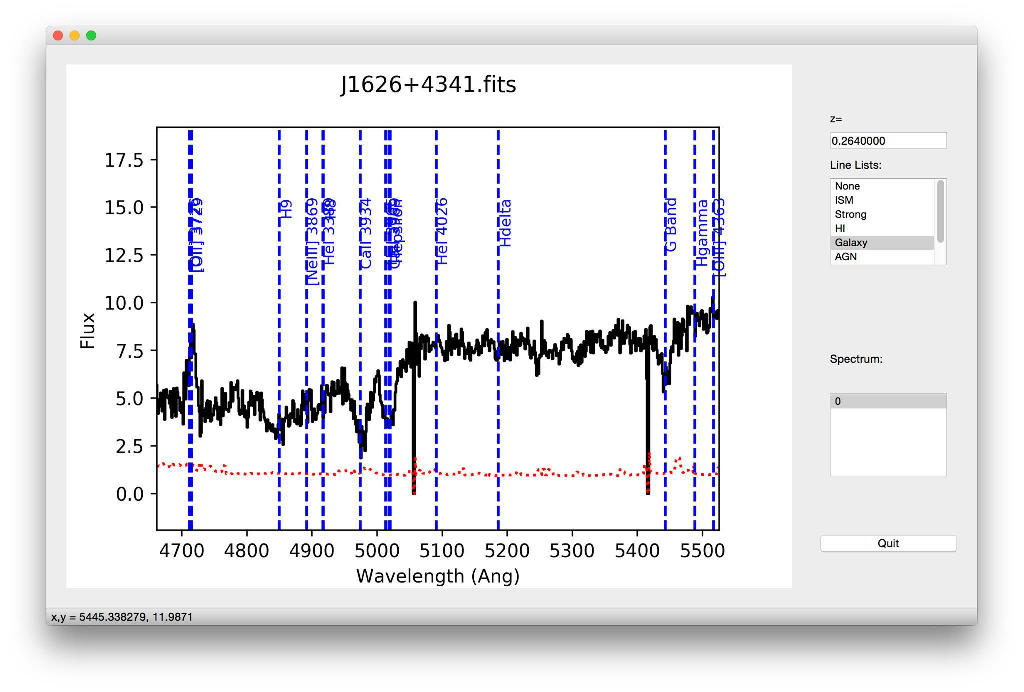
\includegraphics[width=\textwidth]{J1626.pdf}
\caption{
A Kast spectrum of the J1626+4341 galaxy, zoomed into the CaII H+K doublet region. The galaxy has an {\it r}-magnitude 
of 18.3, and a spectroscopic redshift of 0.264. The spectrum is a coadd of three one-hour exposures taken on 2018 Apr 21. 
We mark locations of several common transitions redshifted to the galaxy's frame. 
.}
\label{spectrum}
\end{figure}

\sidecaptionvpos{figure}{c}
\begin{SCfigure}[10][hbt]
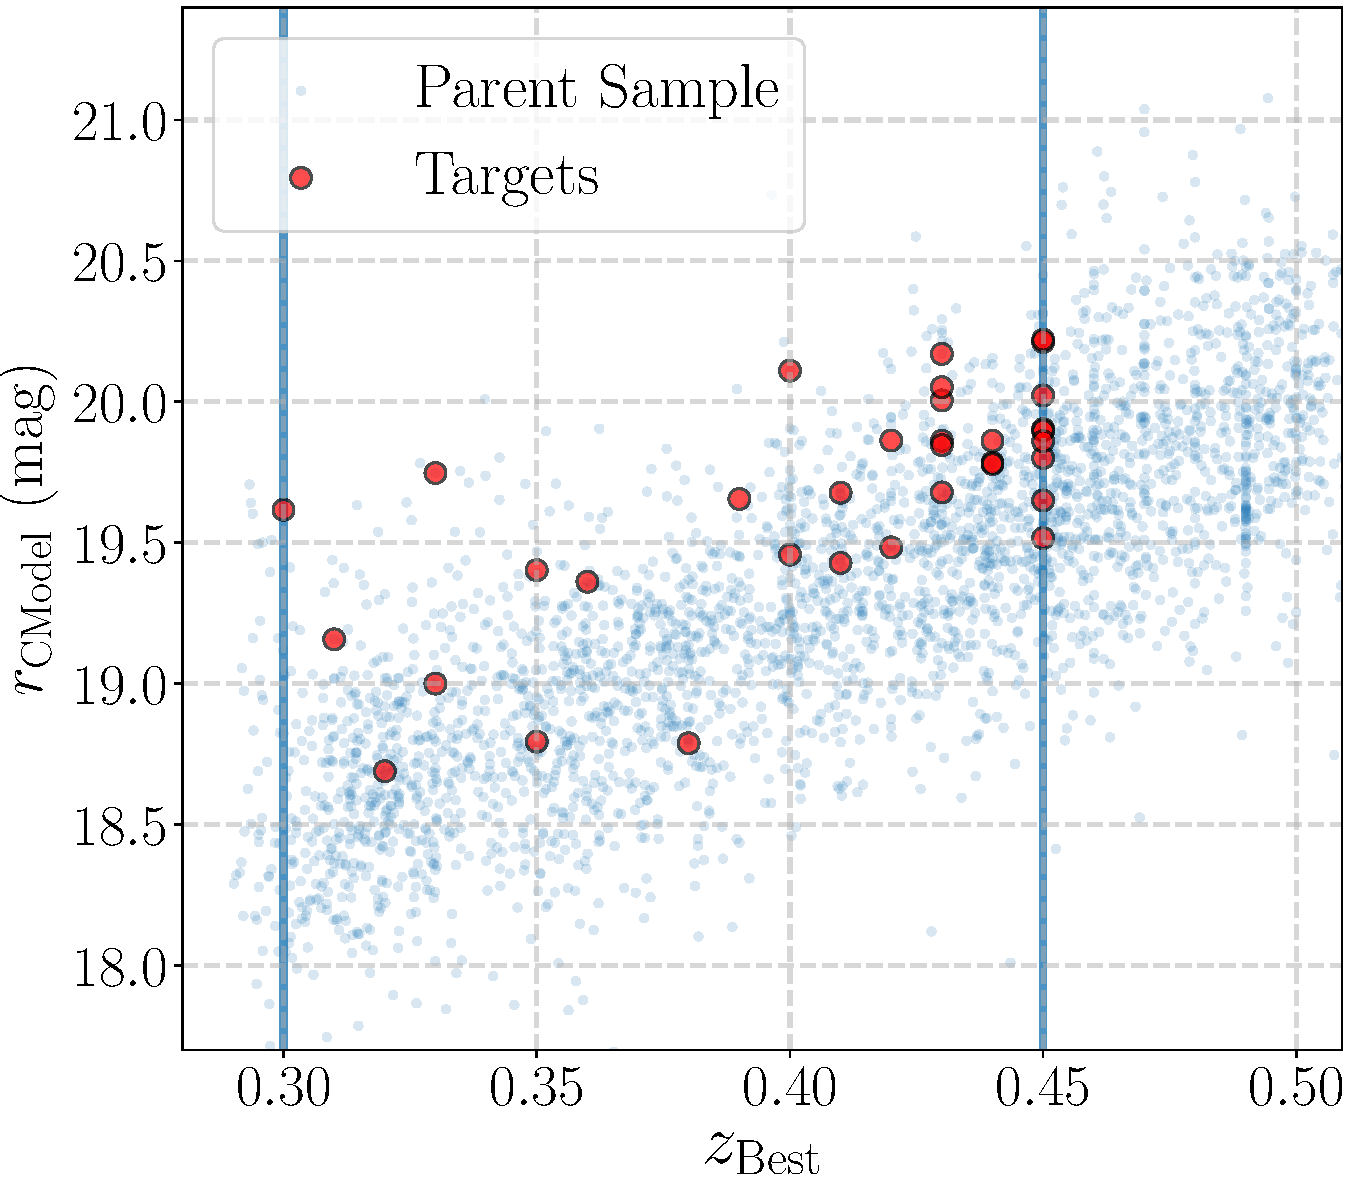
\includegraphics[width=4in]{s16a_massive_photoz_pair_gama_kast_targets.pdf}
\caption{
Distribution of our 2018B targets, as well as the parent HSC survey sample, as a function of redshift and {\it r}-magnitude}
\end{SCfigure}

\begin{figure}[hbt]
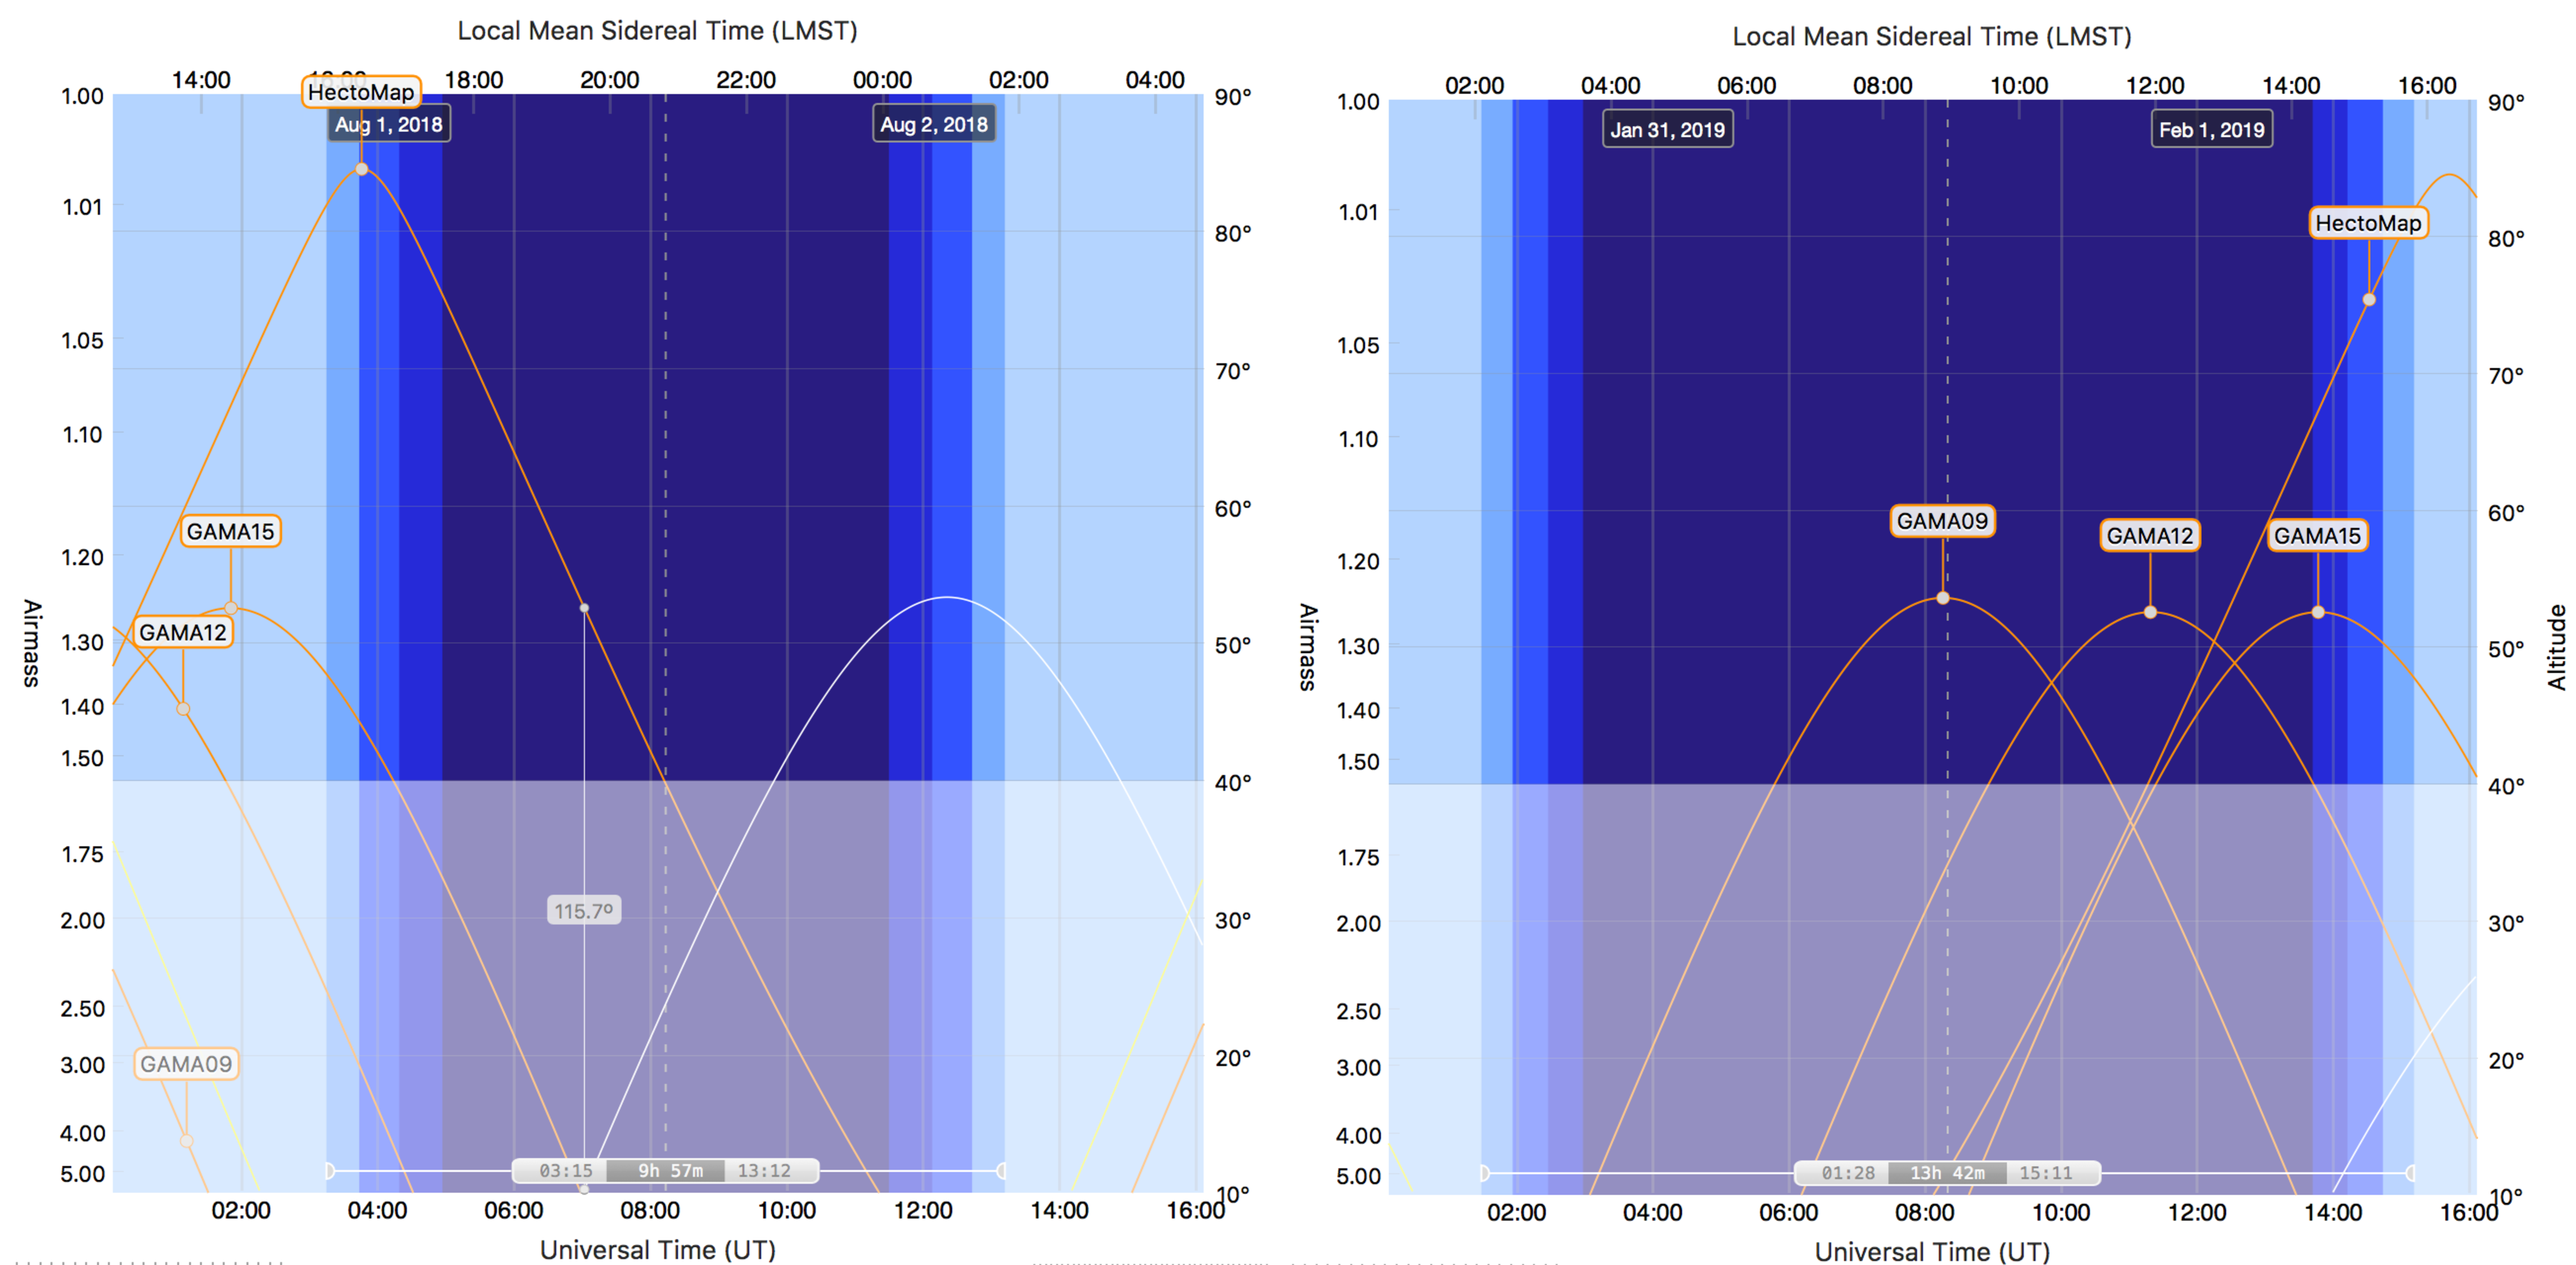
\includegraphics[width=\textwidth]{visibility/2018B.pdf}
\caption{
(Left) Visibility curves of our four targeted fields on 2018 August 1. (Right) Visibility curves on 2019 January 31. We 
request first-half-nights in August, and second-half-nights in January. Our targets will not be visible for more than half 
of the nights in other months.}
\end{figure}

\clearpage

\section{Targets and Exposures}

For this current semester, With Kast observations, we aim at acquiring spectroscopic redshifts of 8 to 14 galaxies in four 
different fields in the sky. Our sample is selected from our HSC catalogs with  $0.25<z_{\rm photo}<0.45$ (our redshift 
range of interest).
We will use the {\it RedRock} software to cross-correlate Kast spectra with galaxy
templates. The distribution of our 2018B targets as well as the parent HSC survey sample in redshift and magnitude are 
shown in Figure~2. 

We were awarded nine nights in 2018A. However, we almost lost our entire program to weather. We have only obtained 
spectroscopic redshift for one galaxy. Figure 1 shows our Kast spectrum of this galaxy, J1626+4341. We reduced the data 
using the PYPIT software. This is the brightest target on our list, with {\it r}-magnitude of 18.3. We attempted 
observing other galaxies on our list, e.g.\ J0857+0131 of {\it r}-magnitude 19.8, and estimated the brightness limit of 
Kast. We find that, for galaxies of $r\sim20$, the object trace 
{\it cannot} be identified on a one-hour Kast red frame at wavelengths $<5000\,\AA$, even under good weather conditions. 
In our 2017 trial run that was director's discretionary time, we observed 
four galaxies that have spectroscopic redshifts already determined from SDSS, to determine the signal-to-noise required 
for deriving reliable spectroscopic redshifts. We find that a signal-to-noise of $>5$ per angstrom is necessary for 
measuring a redshift. A minimum of 
$3\times2\,{\rm hours}=6\,{\rm hours}$ exposure is necessary for faint galaxies of $r\sim20$. As the key features to 
be detected{\textemdash}the CaII H+K doublet and the 4000\,\AA break, 
lie on a steep slope in flux and on the blue end of the Kast red side which has lower efficiency, long exposures are 
required. As the exposure time per frame is long, three frames are necessary for cleaning cosmic rays and alpha particles 
from the dewar. 

Among our four targeted fields, the HectoMap field is visible from dusk until midnight in 2018 August, while the GAMA-09, 
GAMA-12, and GAMA-15 fields are visible from midnight until dawn in 2019 January. Our fields will not be visible in 
other months in 2018B. Therefore, we request first-half-nights in 2018 August and second-half-nights in 2019 January. If 
we are awarded full nights instead, we will supplement the other half of the nights with targets from the J.\ X.\ 
Prochaska research group. Figure~3 shows the visibility curves of the four targeted fields on 2018 August 1 and 2019 
January 31. While dark time is preferred due to the faintness of our targets, our time constraints are more 
critical than dark time.  

We will use the $3''$ slit and the 600/5000 grating on the Kast red side. We will not use the blue side and will take 
out the dichroic beamsplitter. This wide slit will allow more light from our massive, extended galaxies. Our setup will 
resolve and cover the 4000\,\AA\ break, the CaII H and K lines, and the G-band features for a sufficiently wide 
redshift range. 
Our science goal will require 2~hours to 10~hours of exposure per object to obtain sufficient signal-to-noise. These 
long exposures will be broken into one-hour to two-hour exposures, depending on the minimum exposure time required to 
identify the object trace. With overhead, we can observe on average 2 targets per night. Accounting for poor weather 
conditions and Target of Opportunity interrupts, {\bf we request 6 first-half-nights in (early) August and 14 
second-half-nights in (late) January.}

Table~1 lists our galaxies to be observed in 2018B. We will observe the second priority targets if we are granted 
additional observing time. In poor observing conditions we will increase the exposure time and give preference to 
brighter targets. 

\begin{table}
\caption{List of targets.}
\begin{tabular}{ccccccc}
\hline
Name & RA (J2000) & Dec (J2000) & SDSS $r$-mag & photo-$z$ & Exposure (s) & Priority \\
\hline
J0857+0131 & 08:57:06.37 & +01:31:30.7 & 19.8 & 0.42 & 21600 & 1 \\
J1149-0021 & 11:49:48.12 & -00:21:53.6 & 20.4 & 0.43 & 21600 & 1 \\
J1203-0006 & 12:03:46.51 & -00:06:28.2 & 20.2 & 0.42 & 21600 & 1 \\
J1431-0045 & 14:31:33.58 & -00:45:11.2 & 20.3 & 0.43 & 21600 & 1 \\
J1616+4234 & 16:16:49.60 & +42:34:08.9 & 19.6 & 0.43 & 14400 & 1 \\
J1625+4338 & 16:25:24.37 & +43:38:11.0 & 19.6 & 0.40 & 14400 & 1 \\
J1627+4357 & 16:27:36.12 & +43:57:07.4 & 19.5 & 0.41 & 14000 & 1 \\
J1628+4314 & 16:28:29.55 & +43:14:55.7 & 18.9 & 0.38 & 7200 & 1 \\
J0852+0137 & 08:52:57.98 & +01:37:05.6 & 19.9 & 0.44 & 21600 & 2 \\
J0904+0000 & 09:04:08.14 & +00:00:34.1 & 20.1 & 0.42 & 21600 & 2 \\
J1155-0031 & 11:55:11.12 & -00:31:26.6 & 19.1 & 0.33 & 10800 & 2 \\
J1621+4312 & 16:21:59.10 & +43:12:44.8 & 20.2 & 0.44 & 21600 & 2 \\
J1627+4310 & 16:27:38.23 & +43:10:24.0 & 19.2 & 0.44 & 10800 & 2 \\

\end{tabular}
\end{table}

\section{Supplementary Observations Required from other Observatories}

Our full cluster catalogs include spectroscopic redshift catalogs from the GAMA team. We will 
request observing time from Gemini Observatory for targets that are fainter than 
{\it r}-magnitude of 20. 

\section{Technical Remarks}

We have none. 

\subsection{Status of Previously Approved 3-m Programs}

This program obtained director's discretionary time of one night in 2017A, and nine regular 
nights in 2018B. We lost eight out of the nine nights our 2018B program to weather. 

PI Lau is a postdoctoral at UCSC, who has been awarded a total of 32 nights on Shane and has 
been the lead observer of 60 nights on Shane using Kast and ShARCS. 

Co-I Leauthaud and co-I Huang have extensive experience with optical spectroscopy and are experts 
in massive galaxies. 

Co-I Greg Sallaberry is an aspiring undergraduate researcher at UCSC, who will join observing 
and data reduction effort. 

\end{document}

